\newpage
\section{IaaS (Infrastructure as a Service)}
\subsection{Virtualization}
\paragraph{Virtualizzazione} con questo termine si intende la creazione di risorse virtuali come server, spazio di archiviazione o network. Serve per gestire il carico di lavoro rendendo la computazione più \textbf{scalabile}. La forma più comune di virtualizzazione è il \textbf{Server}.\\
La virtualizzazione è un livello di \textbf{astrazione}: il SO è astratto dall'hardware e non è più legato al server/pc dove gira.

\subsubsection{Server Virtualization} Con Server Virtualization si intende il livello di virtualizzazione tra il server fisico e il sistema operativo. Comprende le macchine virtuali sulle quali viene installato il sistema operativo e le applicazioni. Così come il SO permette a tutti i programmi e software di funzionare, il livello di virtualizzazione permette di avere tante macchine virtuali.
\begin{itemize}
    \item \textbf{Virtual Host}: server fisico su cui girano le altre VM
    \item \textbf{Virtual Machine}: ogni SO ospite del Virtual Host
\end{itemize}

\subsubsection{Hypervisor} L'hypervisor è una funzione che crea il livello di virtualizzazione (o \textit{virtualization layer}, permette la virtualizzazione del server) e contiene il Virtual Machine Manager (VMM) per la gestione delle VM.
Il sistema operativo non è installato direttamente sulla macchina ma è astratto dall’hardware: esiste un livello di astrazione tra il server e il sistema operativo chiamato \textbf{virtualization layer} (per esempio ESXi o ESX di VMWare). 
Al livello sopra il virtualization layer ci sono le macchine virtuali, sulle quali è possibile installare un SO.
Esempi di hypervisor: \textit{Vmware Workstation, Virtual Server, Hyper-V , Fusion, XenServer}

\paragraph{Tipi di Hypervisor}
\begin{itemize}
    \item \textbf{Tipo 1}: installato direttamente sull’hardware, e.g. Hyper-V, ESX, ESXi, XenServer
    \item \textbf{Tipo 2}: installato sull’OS dell’hardware come una normale applicazione, e.g. Workstation, Virtual Server, Fusion, Oracle VirtualBox
\end{itemize}
Il tipo 1 è più performante, il tipo 2 non riesce a mantenere più VM contemporaneamente però è più adatto per hardware meno potenti ad esempio un laptop

\subsection{Amazon}
\textbf{Amazon}, fondata inizialmente con il nome di “Cadabra” nel 1994 da Jeff Bezos, era una biblioteca online. Il business plan iniziale era di non aspettarsi profitto per i primi 4-5 anni, il primo profitto lo hanno avuto nel 2001.\\
Ad oggi Amazon detiene quasi il 50\% del mercato Cloud, più precisamente il 47.8\% (seguito da Microsoft 15\%, Alibaba 7\%, Google 4\%). Alcuni dati:
\begin{itemize}
    \item 300 milioni di utenti (Dicembre 2017)
    \item 2 milioni di venditori Amazon (Gennaio 2018)
    \item 560.000 dipendenti (Gennaio 2018)
    \item 3.724 miliardi di dollari di entrate all’anno
\end{itemize}

\subsubsection{Amazon Elastic Compute Cloud (EC2)}
È difficile prevedere il numero di server di cui abbiamo bisogno per un'applicazione, per questo Amazon EC2 mette a disposizione dei server virtuali chiamati \textbf{istanze} configurabili (ad esempio con la scelta di un template Windows/Linux). Si può scegliere tramite Amazon Web Services (\textbf{AWS}) management console (o librerie SDK) la potenza di calcolo delle istanze in base alle proprie necessità. Le istanze si possono scegliere in base a CPU, memoria, storage e GPU.\\
Amazon EC2 ci offre anche un buon livello di sicurezza grazie al \href{https://aws.amazon.com/it/vpc/}{VPC} (Virtual Private Cloud) che rende la connessione più sicura all’interno del Cloud.\\
Inoltre esiste Amazon Elastic Block Store (\textbf{EBS}) che garantisce uno \textbf{storage persistente} per l’uso su EC2, offrendo disponibilità e durabilità dei nostri dati. È stato pensato per le applicazioni che necessitano di big data analytics, stream processing o data warehouse.\\
\textbf{Autoscaling}: Amazon permette di definire delle metriche per decidere come e quando “scalare”, e farlo automaticamente all’occorrenza\\
Per quanto riguarda i \textbf{prezzi}:
\begin{itemize}
    \item \textbf{On demand}: paghi solo per quello che utilizzi (ad esempio prezzo per GB)
    \item \textbf{Reserved instances}: pagamento mensile (cheaper than on-demand), si usa quando si sa già a priori quali e quante macchine serviranno
    \item \textbf{Spot Instances}: sono istanze inutilizzate che Amazon mette in vendita ogni 5 minuti all’asta (fino al 90\% più economiche di quelle on-demand, tipicamente intorno al 50\%)
    \item \textbf{Dedicated hosts}: server fisico con istanze EC2 totalmente dedicato all'utente
    \item \textbf{AWS Free Tier}: livello freemium con limitazioni
\end{itemize}

\subsubsection{Amazon Simple Storage Server (S3)}
Al fine di gestire l’archiviazione dei dati della propria applicazione, Amazon S3 mette a disposizione un servizio di \textbf{storage}. L’interfaccia è estremamente semplice: \textit{drag and drop} in un secchiello (\textbf{bucket}).\\
Amazon S3, per far fronte ad eventuali perdite di dati, esegue 3 backup su 3 unità di memoria diverse e consente di mantenere tutte le vecchie versioni dei file in modo da poterli recuperare se cancellati erroneamente.
Anche per S3 si paga solo quello che si utilizza (\textit{pay per use}).\\
Ci sono diverse  classi di memorizzazione:
\begin{itemize}
    \item \textbf{s3 standard}: oggetti comuni con lettura continua (\$0.023/ GB)
    \item s3 standard \textbf{infrequent access}: accesso poco frequente a questi dati (\$0.012/ GB)
    \item \textbf{Amazon Glacier} per dati da memorizzare a lungo termine, e.g. backup di un database (\$0.004/ GB)
\end{itemize}
Per quanto riguarda i prezzi, si paga per GB e in base alla classe di memorizzazione, ma anche qui si ha un AWS Free Usage Tier con 5GB gratuiti.

\subsection{Dropbox}
Dropbox è stato fondato nel 2007 con l'idea di offrire gratuitamente spazio di archiviazione con limitazioni, con l'opzione di passare al piano premium per avere più storage. A Marzo 2016 Dropbox aveva 500 milioni di utenti.\\
Per i primi 8 anni Dropbox ha sempre usato i server di Amazon S3, (metadati sulle proprie macchine, files su S3) ed era il loro più grande cliente, poi tra il 2014 il 2016 ha costruito le proprie macchine per avere il pieno controllo sui dati. Tuttavia, al momento del passaggio da Amazon S3 ai propri server hanno avuto molti problemi:
\begin{enumerate}
    \item trasferire tutto prima del rinnovo del contratto con Amazon
    \item gli utenti non si sarebbero dovuti accorgere di niente, non avrebbero dovuto avere interruzioni di servizio o perdite di dati nonostante ci volesse 1 giorno intero per trasferire 4 petabyte.
    \item il nuovo software \textit{Magic Pocket} non era totalmente compatibile con il nuovo hardware, hanno dovuto fare delle modifiche rinominandolo \textit{Mozilla Rust}
    \item incidenti stradali per i camion che trasportavano i server hardware
\end{enumerate}

\begin{figure}[h!]
    \centering
    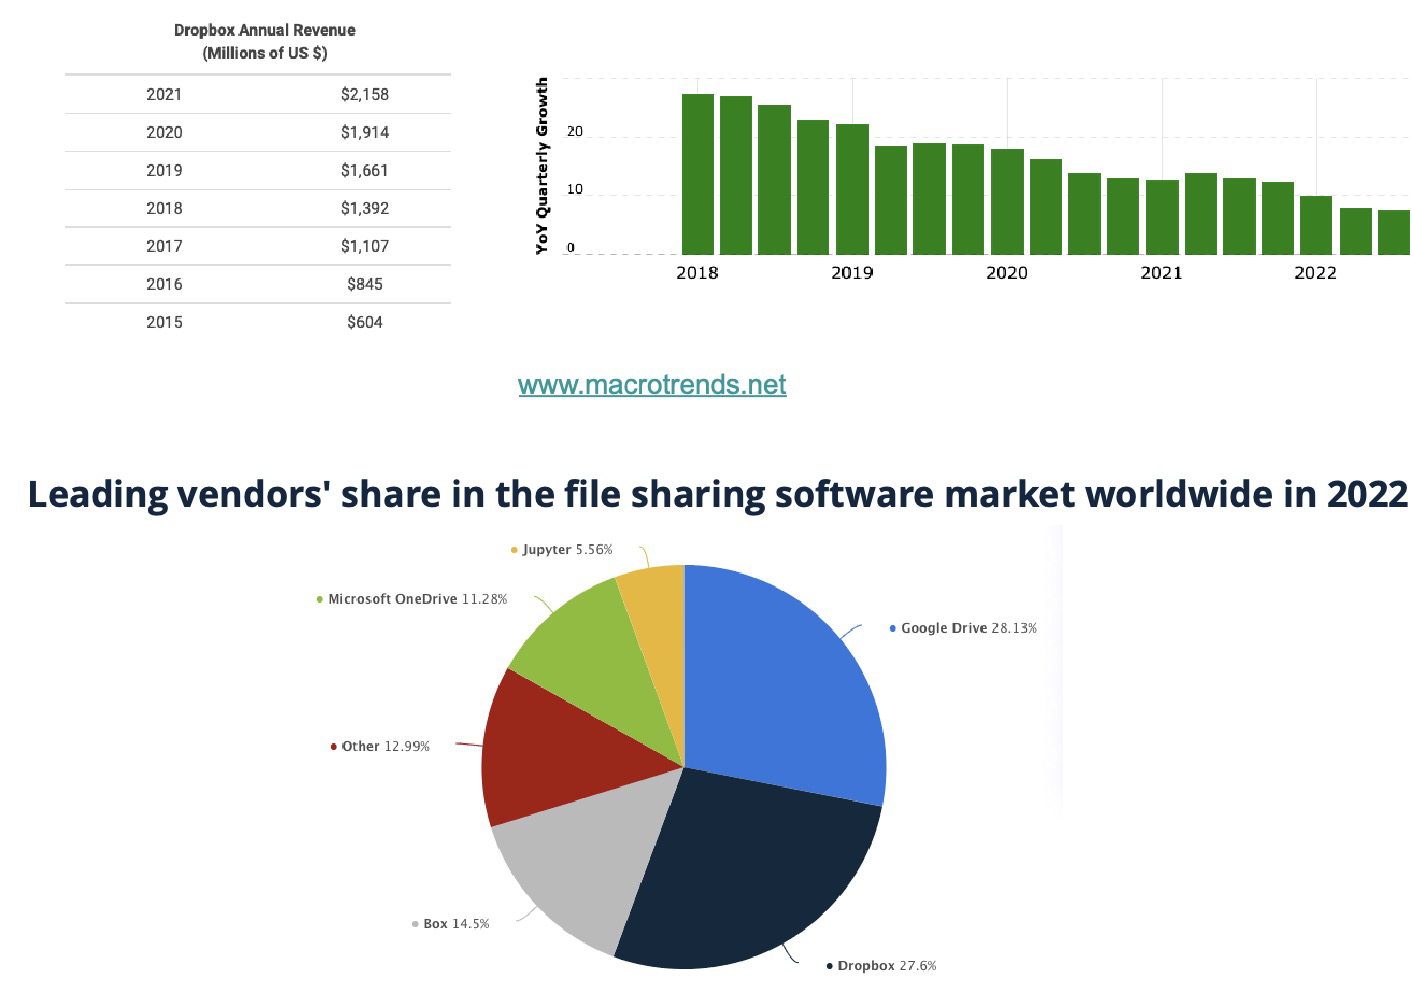
\includegraphics[width=0.7\textwidth]{3.png}
    \caption{Shares del mercato Cloud (2019)}
    %\label{fig:enter-label}
\end{figure}

\paragraph{SLA di Dropbox vs Amazon}
\href{https://aws.amazon.com/agreement}{SLA di AWS} : cosa ci garantisce Amazon? \textbf{Niente}. \textit{The service Offering Are Provided “As is”}.\\
Amazon non dà garanzia riguardo ai servizi offerti, garanzia contrattuale pari a zero.\\
Analogamente il SLA di Dropbox, che non garantisce nessun diritto se ci sono perdite di business, profitto o dati.

\newpage
\paragraph{Come suddividere un’applicazione three-tier su un Cloud ibrido?} 
\begin{enumerate}
    \item Web server (presentation tier)
    \item App server (business logic tier)
    \item DB server (data tier)
\end{enumerate}
In generale qualsiasi soluzione va bene, solitamente si mettono almeno 2 parti sul Cloud pubblico, in alcuni casi anche tutto. Più raramente viene usato solo il Cloud privato.

\subsection{AWS IAM}
AWS IAM  (\textbf{I}dentity and \textbf{A}ccess \textbf{M}anagement) permette di controllare e gestire l'accesso degli utenti ai servizi AWS. IAM consente di creare utenti, gruppi di utenti e policy di autorizzazione per controllare quale operazione può essere eseguita da ogni utente o gruppo. In questo modo è garantito che solo utenti autorizzati possano accedere e gestire determinate risorse.\\
In particolare, IAM permette di:
\begin{itemize}
    \item gesitre gli utenti di IAM e i loro accessi
    \item gestire ruoli e permessi
    \item autenticazione federata: accedere autenticandosi tramite Google
\end{itemize}

\paragraph{Access management} che cosa ha diritto di fare un utente dopo che si è autenticato, e.g. quali dati può vedere e quali può modificare
L' autenticazione  ad IAM si può effettuare tramite la GUI della dashboard, tramite CLI di AWS o tramite kit di development (SDK)
\begin{figure}[h!]
    \centering
    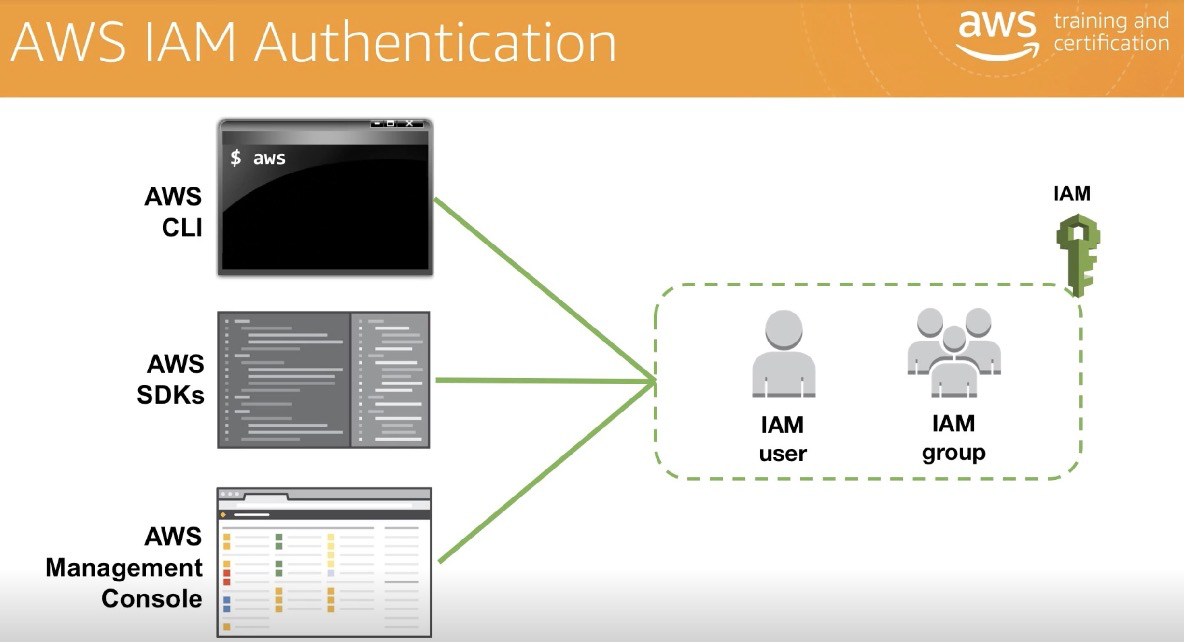
\includegraphics[width=0.6\textwidth]{4.png}
    \caption{Possibili metodi di autenticazione con AWS IAM}
    \label{fig:enter-label}
\end{figure}
\newpage
I  permessi  di IAM sono definiti tramite  \textbf{policy} , che non sono altro dei file \textbf{JSON} in cui sono salvati i permessi degli utenti. Uno use-case è ad esempio quando si crea un bucket si può associare una policy di pieno accesso/read only alle risorse
\begin{figure}[h!]
    \centering
    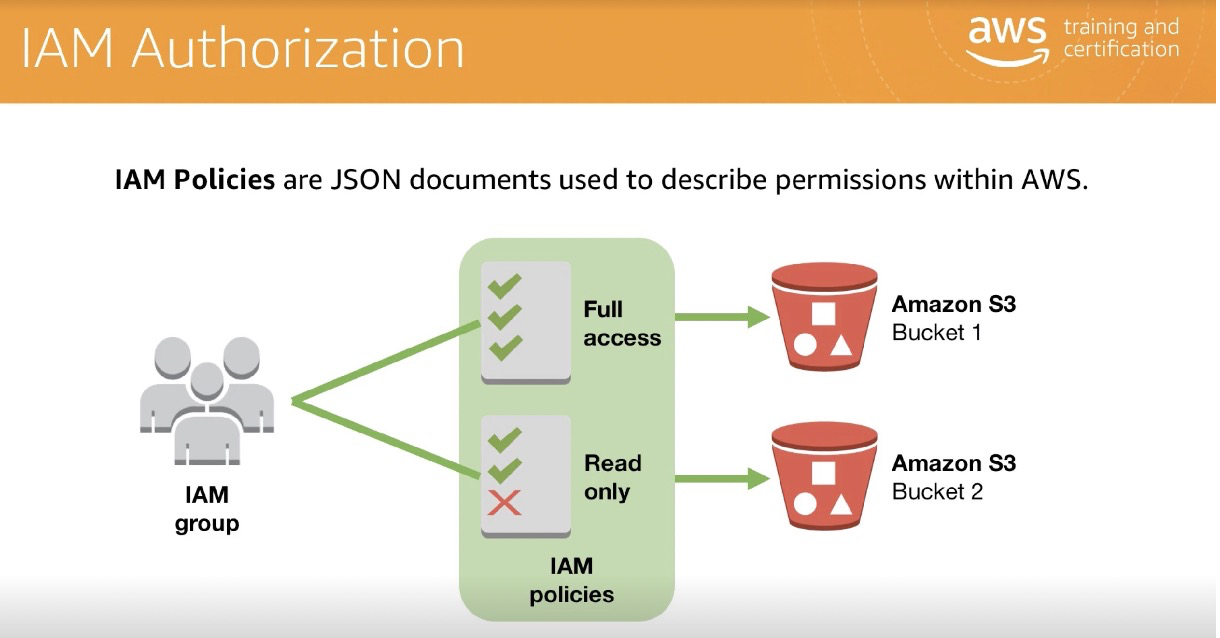
\includegraphics[width=0.6\textwidth]{5.png}
    \caption{IAM group}
    \label{fig:enter-label}
\end{figure}

Infine, IAM permette anche di creare gruppi di utenti e utenti individuali e assegnare dei ruoli a determinati gruppi/individui
\begin{figure}[h!]
    \centering
    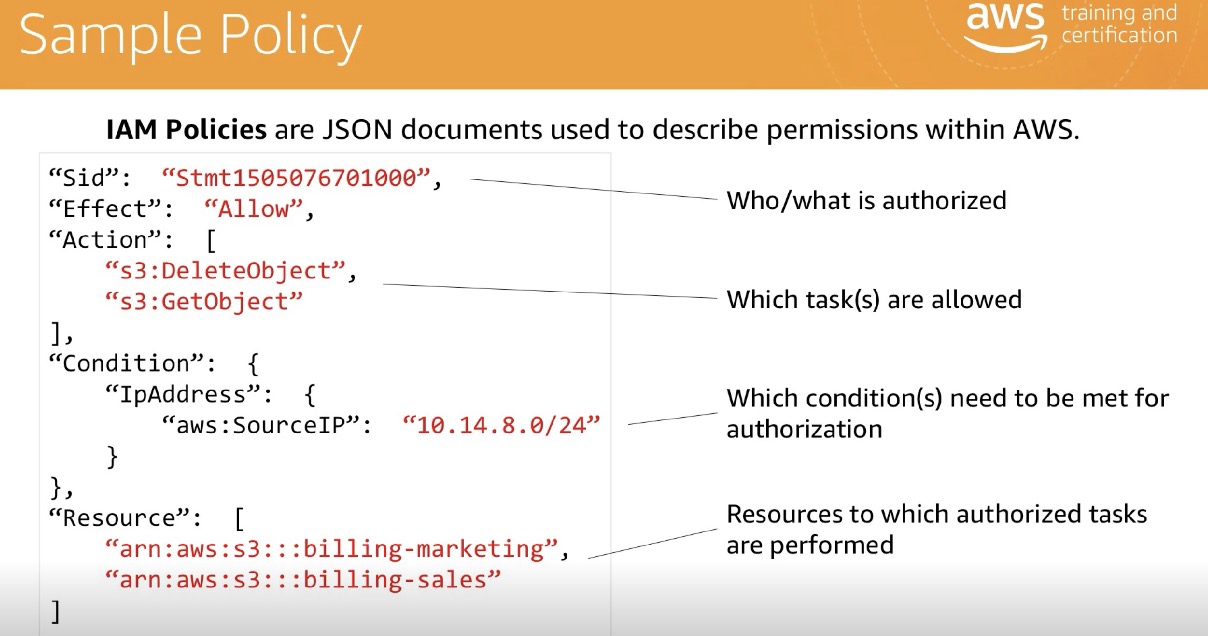
\includegraphics[width=0.6\textwidth]{6.png}
    \caption{IAM Policies, file JSON per gestire i permessi e l'accesso alle risorse}
    \label{fig:enter-label}
\end{figure}